\chapter{Introduction}
\label{C:intro}

\begin{figure}[t]
\centering
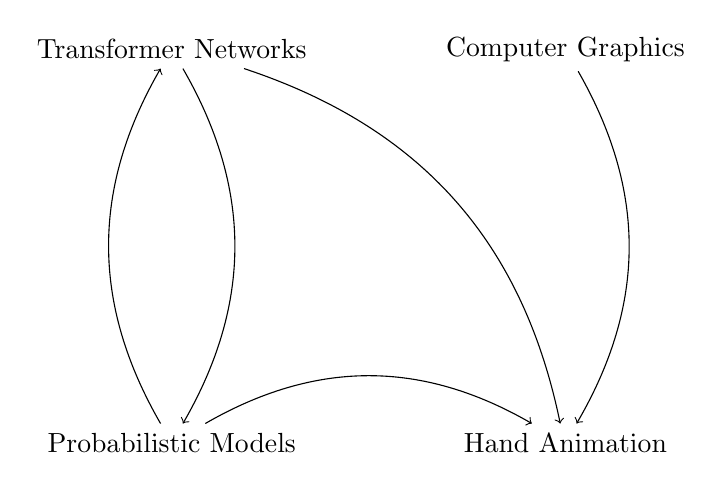
\begin{tikzpicture}
    \tikzstyle{every node}=[node distance=5cm]
    \node (tn) {Transformer Networks};
    \node (pm) [below of=tn] {Probabilistic Models};
    \node (cg) [right of=tn] {Computer Graphics};
    \node (an) [below of=cg] {Hand Animation};

    \draw[->,bend left] (tn) to (pm);
    \draw[->,bend left] (pm) to (tn);
    \draw[->,bend left] (cg) to (an);
    \draw[->,bend left] (pm) to (an);
    \draw[->,bend left] (tn) to (an);
\end{tikzpicture}
\caption[The relationship between the different fields in this thesis]{How learnings and experiments from different fields contribute to each other in this thesis.}
\end{figure}

This thesis introduces concepts and experiments at the intersection of two areas: Deep Learning and Computer Graphics. There are three main areas of focus: Comprehensively introducing a class of neural network models called \textit{transformer} networks; an experiment comparing different sampling orders when predicting data using\textit{auto-regressive} transformer models; and the developement of an application of auto-regressive transformer models for \textit{hand pose modeling}.

\section{Contributions}

Although much of the work done is summarizing others' research and presenting learnings, there are two main novel contributions:
\begin{enumerate}
    \item I present experiments with \textit{dynamically-ordered} auto-regressive sampling, utilising the \textit{permutation-invariance} property of the attention operation in transformer models.
    \item I present a proof-of-concept transformer-based generative model for hand motion prediction, which can be used to predict hand motion at arbitrary target frames, and to predict the joints of a hand in any order within that frame.
\end{enumerate}
These contributions involved training neural networks (see \Cref{fig:context}), in particular transformers, on two datasets - MNIST, and a motion capture dataset of hand motion. The results of these experiments are presented in \Cref{C:a-o-sampling} and \Cref{C:hand-model} respectively.

\begin{figure}
    \centering
    
\pgfdeclarelayer{bg}
\pgfsetlayers{bg,main}

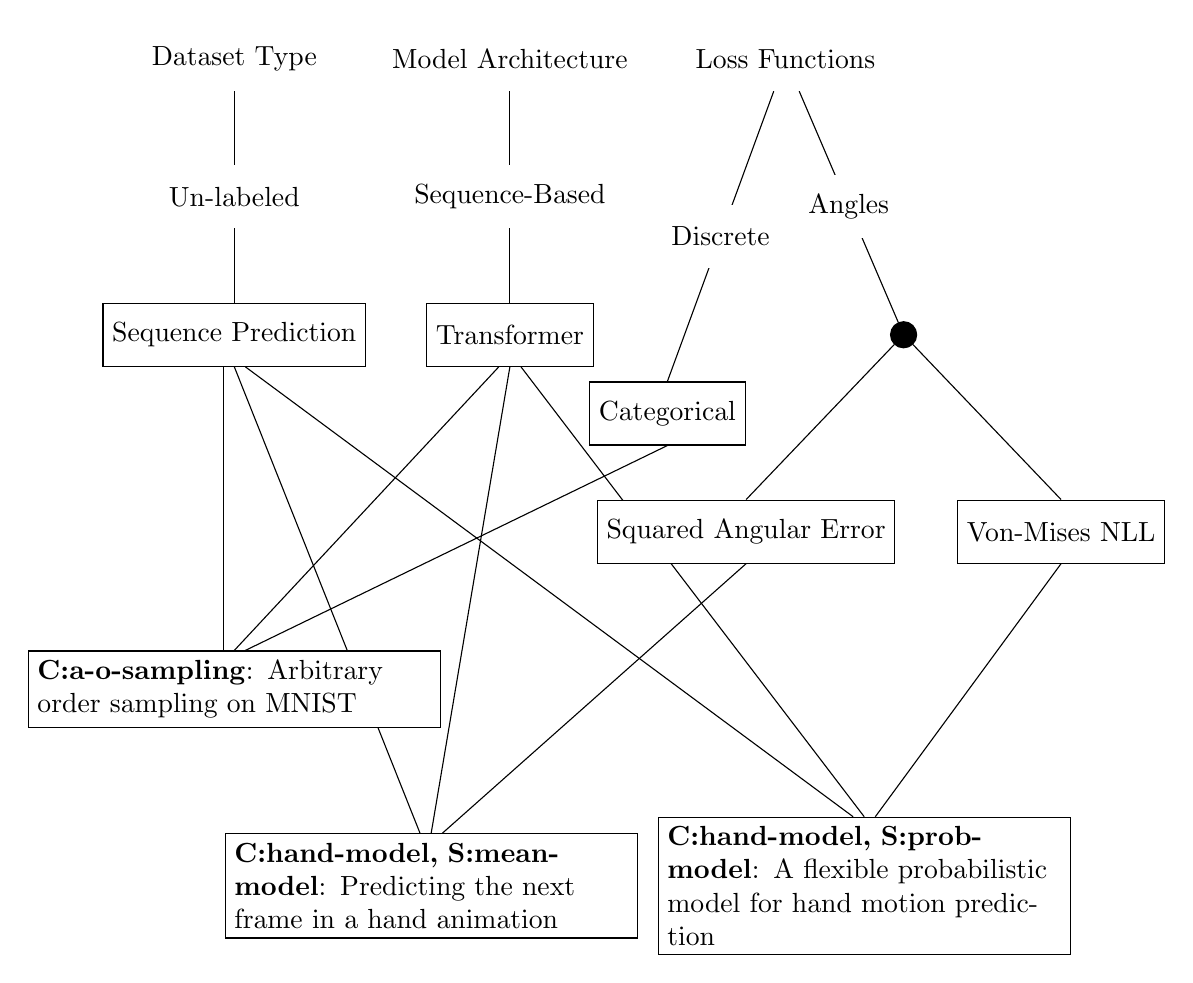
\begin{tikzpicture}
    \tikzstyle{every node}=[node distance=3.5cm,minimum height=0.8cm]

    % dataset type
    \node (datasettype) {Dataset Type};
    \node[draw, below of=datasettype] (seqpred) {Sequence Prediction};
    \draw (datasettype) -- node[fill=white] {Un-labeled} (seqpred);

    % input shape
    \node[right of=datasettype] (seqmodel) {Model Architecture};

    % loss
    \node[right of=seqmodel] (loss) {Loss Functions};

    % angles
    \node[draw,fill=black,minimum height=0.2cm,circle,below of=loss,xshift=1.5cm] (angles) {};
    \draw (loss) -- node[fill=white] {Angles} (angles);

    \node[draw,fill=white,below of=angles,node distance=2.5cm, xshift=-2cm] (amse) {Squared Angular Error};
    \draw (angles) -- (amse.north);

    \node[draw,fill=white,below of=angles,node distance=2.5cm, xshift=2cm] (vonmises) {Von-Mises NLL};
    \draw (angles) -- (vonmises.north);

    \node[draw,fill=white,below of=loss,node distance=4.5cm,xshift=-1.5cm] (cat)  {Categorical};
    \draw (loss) -- node[fill=white] {Discrete} (cat.north);

    % transformer (here because needs to draw above a line)
    \node[draw, below of=seqmodel] (transformer) {Transformer};
    \draw (seqmodel) -- node[fill=white] {Sequence-Based} (transformer);


    % chapter 4: arbitrary order sampling
    \node[draw,fill=white,text width=5cm] (chapter4) at (0,-8cm) {\textbf{\Cref{C:a-o-sampling}}: Arbitrary order sampling on MNIST};

    % chapter 6.2: transformer for hand pose prediction
    \node[draw,fill=white,text width=5cm] (chapter62) at (2.5cm,-10.5cm) {\textbf{\Cref{C:hand-model}, \Cref{S:mean-model}}: Predicting the next frame in a hand animation};

    % chapter 6.3: probabilistic model for hand pose prediction
    \node[draw,fill=white,text width=5cm] (chapter63) at (8cm,-10.5cm) {\textbf{\Cref{C:hand-model}, \Cref{S:prob-model}}: A flexible probabilistic model for hand motion prediction};

    \begin{pgfonlayer}{bg}
        \draw ([xshift=-4pt]seqpred.south) -- ([xshift=-4pt]chapter4.north);
        \draw ([xshift=-4pt]transformer.south) -- (chapter4.north);
        \draw (cat.south) -- ([xshift=4pt]chapter4.north);

        \draw (seqpred.south) -- ([xshift=-4pt]chapter62.north);
        \draw (transformer.south) -- (chapter62.north);
        \draw (amse.south) -- ([xshift=4pt]chapter62.north);

        \draw ([xshift=4pt]seqpred.south) -- ([xshift=-4pt]chapter63.north);
        \draw ([xshift=4pt]transformer.south) -- (chapter63.north);
        \draw (vonmises.south) -- ([xshift=4pt]chapter63.north);
    \end{pgfonlayer}
\end{tikzpicture}

    \vspace{1cm}
    \captionsetup{parskip=7pt}
    \caption[Where my work sits.]{The later work in this thesis sits focuses on learning un-labeled sequence data with transformers, in two different domains.

    In \Cref{C:a-o-sampling}, I train a transformer-based probabilistic model which can be used as a gaussian process for predicting pixels on the MNIST dataset.

    In \Cref{C:hand-model}, I train a transformer-based model on the ManipNet hand motion dataset. \Cref{S:mean-model} focuses on a deterministic model, while \Cref{S:prob-model} focuses on a probabilistic model.}
    \label{fig:context}
\end{figure}

\section{Structure}

The structure of the remainder of this thesis is as follows:

\begin{enumerate}
    \item \Cref{C:background} \nameCref{C:background} introduces notation and concepts for neural networks which will be used throughout the thesis.

    \item \Cref{C:transformers} provides an introduction and literature reivew of a class of neural network models called \textit{transformers}, which are a class of models that have become very broadly used in the past few years.

    \item \Cref{C:a-o-sampling} presents a novel method for sampling sequence data in an arbitrary order, including a pretraining task variant, and experiments with this method with transformer models on the MNIST dataset.

    \item \Cref{C:angles-joints-hands} introduces notation and concepts for the problem domain of \textit{hand motion modeling}, including methods for representing and working with joint angles and rotations, and character/hand pose data.

    \item \Cref{C:hand-model} then presents the development of a transformer model for predicting hand pose data and generating animations of hands.

    \item Lastly, \Cref{C:conclusion} summarizes the thesis and discusses future work and reflections.
\end{enumerate}
